%!TEX root=../GaugeCNNTheory.tex


\subsection{Parallel transport of feature vectors}
\label{sec:transport_local}

The kernels of convolutional networks accumulate features from all points $q$ in a neighborhood around each point $p$ of the manifold.
Since features at different points live in different feature vector spaces and are expressed relative to different gauges, they need to be \emph{parallel transported} along some path $\gamma$ from $q$ to $p$ before they can be processed further.
We first discuss the transport of tangent vectors, which is formalized by a parallel transport map
\begin{align}
    \mathcal{P}_\gamma: \TqM \to \TpM \,.
\end{align}
This transporter is often computed from the canonical Levi-Civita connection of the manifold, however, it might in some applications correspond to an alternative ($G$-compatible) connection, as further discussed below and in our literature review in Part~\ref{part:literature_review}.
A transporter of ($G$-associated) feature vectors follows from that of the tangent vectors if the transport is $G$-compatible.




\subsubsection{Tangent vector transporters}

It is didactically reasonable to start with the specific case of Levi-Civita transporters on Euclidean spaces, depicted in Fig.~\ref{fig:transport_flat}, before proceeding to more general transporters and manifolds.
In this case the parallel transport is independent from the chosen path $\gamma$ and keeps the transported vector parallel in the usual sense on Euclidean spaces.
Note that the transporter~$\mathcal{P}_\gamma$ is mapping between the tangent spaces $\TqM$ and $\TpM$ and is therefore coordinate free.
It can, however, be expressed relative to coordinates, then operating on numerical coefficient vectors instead of tangent vectors.
An intuition is given in Fig.~\ref{fig:transport_flat}, where the frames at $q$ and $p$ are not parallel%
\footnote{
    In contrast to general manifolds, $\R^d$ comes with a canonical notion of parallelism of reference frames.
}
such that the coefficients $(1,1)^\top$ at $q$ and $\big(\sqrt{2},0\big)^\top$ at $p$ differ even though the corresponding (coordinate free) tangent vectors are parallel to each other.
To make this more precise, consider gauges $\psi_q^{\widetilde{A}}$ and $\psi_p^A$ to be given on neighborhoods $U^{\widetilde{A}}$ of $q$ (red) and $U^A$ of $p$ (green).
Let a vector $v = \big( \psi_q^{\widetilde{A}} \big)^{-1} (v^{\widetilde{A}}) \in \TqM$ be given by its coefficients $v^{\widetilde{A}} \in \R^d$.
The coefficients of the transported vector $\mathcal{P}_\gamma v$ at $p$ are then given by
$
\psi_p^A \circ \mathcal{P}_\gamma (v)
\ =\ \psi_p^A \circ \mathcal{P}_\gamma \circ \big(\psi_q^{\widetilde{A}}\big)^{-1} (v^{\widetilde{A}})
$.
It follows that the coordinate expression of a transporter is relative to gauges $\widetilde{A}$ and $A$ expressed as:%
\footnote{
    $g_\gamma^{A\widetilde{A}}$ takes values in $\GL{d}$ if we assume arbitrary ($\mathfrak{gl}(d)$-valued) connections and general structure groups $G\leq\GL{d}$.
    For the $\mathfrak{so}(d)$-valued Levi-Civita connection and orthonormal frames, i.e. $G=\O{d}$, one has $g_\gamma^{A\widetilde{A}} \in \O{d}$.
}
\begin{align}\label{eq:transporter_gauge}
    g_\gamma^{A\widetilde{A}} \ :=\ \psi_p^A \circ \mathcal{P}_\gamma \circ \big( \psi_q^{\widetilde{A}} \mkern1mu\big)^{-1} \in\, \GL{d}
\end{align}
The group element $g_\gamma^{A\widetilde{A}}$ accounts for non-parallel choices of reference frames at $q$ and $p$.
On $\R^d$, one typically assumes all frames to be parallel such that all coordinatizations of Levi-Civita transporters become trivial.%
\footnote{
    Conventional CNNs on $\R^d$ implicitly make this assumption of parallel frames (Fig.~\ref{fig:G_structure_intro_a}) and trivial transporters.
}

\begin{figure*}
    \centering
    \begin{subfigure}[b]{0.5\textwidth}
        \centering
        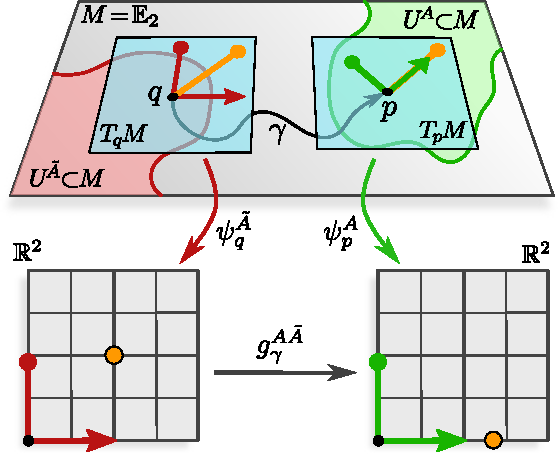
\includegraphics[width=.95\textwidth]{figures/transport_flat.pdf}
        \vspace*{1ex}
        \caption{\small
            Parallel transport and its coordinatization on a flat space.
        }
        \label{fig:transport_flat}
    \end{subfigure}
    \hfill
    \begin{subfigure}[b]{0.4\textwidth}
        \centering
        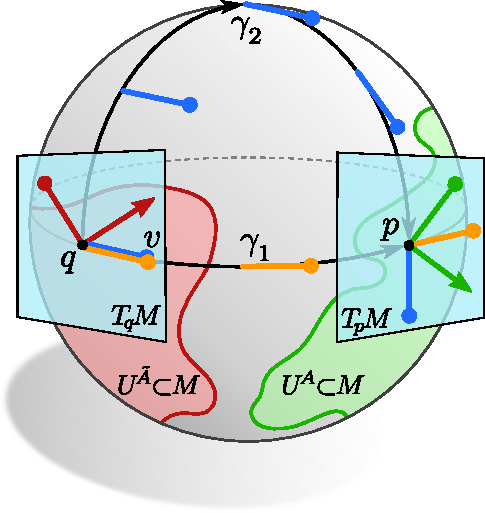
\includegraphics[width=\textwidth]{figures/transport_sphere.pdf}
        \vspace*{-2ex}
        \caption{\small
            Parallel transport on the 2-sphere $S^2$.
        }
        \label{fig:transport_sphere}
    \end{subfigure}
    \caption{\small
        Parallel transport of tangent vectors $v\in \TqM$ at $q$ to $\mathcal{P}_\gamma v \in \TpM$ at $p$.
        Fig.~\ref{fig:transport_flat} visualizes the special case of Levi-Civita transporters on flat Euclidean spaces $M = \Euc_2$.
        Independently from the chosen path $\gamma$, the Levi-Civita transport keeps the vector (orange) parallel in the usual sense in Euclidean spaces.
        Gauges $\psi_q^{\widetilde{A}}$ (red) and $\psi_p^A$ (green) allow to express the coordinate free transporter by a group element
        $g_\gamma^{A\widetilde{A}} = \psi_p^A \circ \mathcal{P}_\gamma \circ \big(\psi_q^{\widetilde{A}}\big)^{-1} \in \GL{d}$
        which accounts for the change of vector coefficients if the target frame does not agree with the transported source frame.
        Fig.~\ref{fig:transport_sphere} shows the Levi-Civita transport on the 2-sphere~$S^2$, Eq.~\eqref{eq:sphere_transport_embedded}.
        The transporters $\mathcal{P}_{\mkern-2mu\gamma_1}$ and $\mathcal{P}_{\mkern-2mu\gamma_2}$ along different paths $\gamma_1$ and $\gamma_2$ disagree in general.
        As before, the coordinate free transporters can be expressed by group elements that operate on coefficients relative to the coordinate frames at $q$ and $p$.
     }
    \label{fig:transport}
\end{figure*}


As the transporter in Eq.~\eqref{eq:transporter_gauge} is coordinate dependent, we are interested in its gauge transformations.
Denote by $\psi_q^{\widetilde{B}}$ and $\psi_p^B$ two alternative gauges on neighborhoods of $q$ and $p$.
From the commutative diagram
\begin{equation}\label{cd:transporter_trivialization}
\begin{tikzcd}[column sep=50pt, row sep=25pt, font=\normalsize]
    \R^d
        \arrow[dd, "g_q^{\widetilde{B}\widetilde{A}}\cdot\ "']
        \arrow[rrr, "g_\gamma^{A\widetilde{A}}\cdot"]
    & &[-1ex] &
    \R^d
        \arrow[dd, "\ g_p^{BA}\cdot"]
    \\
    &
    \TqM
        \arrow[ul, "\psi_q^{\widetilde{A}}"]
        \arrow[dl, "\psi_q^{\widetilde{B}}"']
        \arrow[r, "\mathcal{P}_\gamma"]
    &
    \TpM
        \arrow[ur, "\psi_p^A"']
        \arrow[dr, "\psi_p^B"]
    \\
    \R^d
        \arrow[rrr, "g_\gamma^{B\widetilde{B}}\cdot"']
    & & &
    \R^d
\end{tikzcd}
\end{equation}
one can then read off that the transporters in the different gauges are related by
\begin{align}\label{eq:transporter_gauge_trafo}
    g_\gamma^{B\widetilde{B}}
    \ =\ g_p^{BA}\, g_\gamma^{A\widetilde{A}}\, \big(g_q^{\widetilde{B}\widetilde{A}} \mkern1mu\big)^{-1}
\end{align}
Note the similarity of this transformation law and commutative diagram to those in Eqs.~\eqref{eq:matrix_gaugetrafo} and~\eqref{eq:linear_map_TpM_diagram}.
The difference between both is that the transporter has a different domain $\TqM$ and codomain $\TpM$, which are trivialized by different, independent gauges and transform therefore independently.


In general, the parallel transport of tangent vectors is determined by some choice of connection, for instance (but not necessarily) by the canonical Levi-Civita connection of a Riemannian manifold.
A connection can be seen as a collection of infinitesimal transporters between adjacent tangent spaces, such that the full transporter $\mathcal{P}_\gamma$ is given by integrating the connection along the path $\gamma$.
The transporters along different paths $\gamma_1$ and~$\gamma_2$ from $q$ to~$p$ need not agree, which is in Fig.~\ref{fig:transport_sphere} exemplified by Levi-Civita transporters on the 2-sphere~$S^2$, cf.~Eq.~\eqref{eq:sphere_transport_embedded}.
As for flat spaces, the coordinate free transporters can by Eq.~\eqref{eq:transporter_gauge} be expressed relative to gauges.
The gauge transformations of such coordinatized transporters are again given by Eq.~\eqref{eq:transporter_gauge_trafo}.
The transporters on a given manifold can in principle be calculated analytically from the connection~\cite{gallier2019diffgeom1,nakahara2003geometry} and can sometimes be expressed in closed form, for instance for the sphere $S^2$, Eq.~\eqref{eq:sphere_transport_embedded}.
Several numerical algorithms exist to compute parallel transporters on meshes; see Section~\ref{sec:surfaces_geom_mesh}.
We will not go into more details on how to compute tangent vector transporters $\mathcal{P}_\gamma$ but simply assume them to be given.




\subsubsection{Feature vector transporters}

Eq.~\eqref{eq:gauge_trafo_features} defines the transformation law of feature vector coefficients by their \emph{field type}~$\rho$.
Their parallel transporter, expressed relative to gauges $\psi_q^{\widetilde{A}}$ and $\psi_p^A$, is analogously given by wrapping the tangent vector coefficient transporter into this field representation, that is, by
\begin{align}
    \rho\big( g_\gamma^{A\widetilde{A}} \big) \,.
\end{align}
Note that -- since $\rho:G\to\GL{c}$ is a $G$-representation -- this construction is only then well defined when all transporters~$g_\gamma^{A\widetilde{A}}$ (for arbitrary paths $\gamma$ and frames $A$, $\widetilde{A}$) are actually taking values in the chosen structure group~$G$.
Whether this is the case depends both on the particular choice of $G$-structure (or $G$-atlas) and the transporters (or connection) considered -- they need to be \emph{compatible}~\cite{wendlLectureNotesBundles2008}.


All convolutional networks accumulate (thus transport) feature vectors in one way or the other, and assume therefore some choice of connection and $G$-structure.
If the chosen $G$-structure is incompatible with the Levi-Civita connection, this implies that these models are -- often implicitly -- assuming an alternative, $G$-compatible connection to accumulate features.
The reader should for now not worry about the specific choices of connections, which will become more clear in our literature review in Part~\ref{part:literature_review}.
In the remainder of this section, we will elaborate more on the $G$-compatibility of connections and $G$-structures.
Assuming that \emph{feature transporters will in the following always be well defined}, this part can be safely ignored at a first reading.

A more rigorous, coordinate free discussion of transporters on the associated feature vector bundles can be found in Section~\ref{sec:bundle_transport}.






\subsubsection{Compatibility of connections and \textit{G}-structures}

A connection is said to be \emph{$G$-compatible} with a $G$-structure $\GM$ if the coordinate expressions $g_\gamma^{A\widetilde{A}}$ of its transporters $\mathcal{P}_\gamma$ relative to any frames $A$, $\widetilde{A}$ of $\GM$ take values in the structure group~$G$~\cite{wendlLectureNotesBundles2008}.%
\footnote{
    Equivalently, the \emph{connection 1-form} of the connection, expressed relative to frames of $\GM$, is required to be $\mathfrak{g}$-valued, where $\mathfrak{g}$ denotes the Lie algebra of~$G$.
    More abstractly, we are interested in \emph{principal Ehresmann connections} on the principal $G$-bundle $\GM$.
}
A $G$-compatible connection gives rise to transporters of $G$-associated feature vectors.

To illuminate this somewhat abstract compatibility condition, we discuss a few specific examples.
A simple example is that of the Levi-Civita connection on $\R^2$, Fig.~\ref{fig:transport_flat}, 
Consider the two $\{e\}$-structures on $\R^2$ that are shown in Figs.~\ref{fig:frame_field_automorphism_1} and~\ref{fig:frame_field_automorphism_2}.
Here $G=\{e\}$, which means that the field type $\rho: \{e\} \to \GL{c}$ is a $\{e\}$-representation, such that the parallel transport of feature vectors can only be defined if the coordinate expressions $g_\gamma^{A\widetilde{A}}$ take values in~$\{e\}$, i.e. are trivial.
As the $\{e\}$-structure in Fig.~\ref{fig:frame_field_automorphism_1} consists of ``parallel'' frames, this is indeed the case -- the Levi-Civita connection is thus compatible with this $\{e\}$-structure.
In contrast, the frames of the $\{e\}$-structure in Fig.~\ref{fig:frame_field_automorphism_2} are ``rotated'' relative to each other, resulting in non-trivial coordinate expressions $g_\gamma^{A\widetilde{A}}$ that take values in $\SO2$ (visualized in Fig.~\ref{fig:transport_flat}).
Since the field type $\rho: \{e\} \to \GL{c}$ does not handle rotations, it is not possible to define the Levi-Civita transport of features associated to this $\{e\}$-structure -- they are incompatible.
As a second example, consider the Levi-Civita connection on $S^2$, shown in Fig.~\ref{fig:transport_sphere}.
The transport will in this case always be path dependent and lead to differently rotated vectors, implying that $g_\gamma^{A\widetilde{A}}$ will take values in $\SO2$.
Feature vectors to be transported according to Levi-Civita connection need therefore to be of some type $\rho: \SO2 \to \GL{c}$ that is an $\SO2$-representations.
This requires at least the $\SO2$-structure on $S^2$ that is shown in Fig.~\ref{fig:G_structure_S2_1}.
The $\{e\}$-structure on $S^2$ from Fig.~\ref{fig:G_structure_S2_2} is incompatible with the Levi-Civita connection.


Since the Levi-Civita connection is a metric connection, it preserves lengths of and angles between tangent vectors, and thus transports orthonormal frames to orthonormal frames.
It follows that the Levi-Civita connection is \emph{always} compatible with the $\O{d}$-structure of orthonormal frames, relative to which $g_\gamma^{A\widetilde{A}}$ takes values in~$\O{d}$.
If the manifold is orientable, the frame-handedness is preserved by Levi-Civita transporters, which means that they are guaranteed to be compatible with $\SO{d}$-structures of orthonormal, right-handed frames on~$M$.
All of the convolutional networks in our literature review in Part~\ref{part:literature_review} that are based on $\SO{d}$-structures accumulate features via Levi-Civita transporters.


If a given $G$-structure is incompatible with the Levi-Civita connection, one needs to define an alternative, $G$-compatible connection to transport the feature vectors.
The most prominent example in our literature review is that of \emph{trivial connections} on $\{e\}$-structures.
A trivial connection is characterized by the property that its transport is \emph{path independent}~\cite{craneTrivialConnectionsDiscrete2010}.
Any $\{e\}$-structure implies a unique trivial connection, which transports tangent vectors such that they keep the same angle to the reference frames of the $\{e\}$-structure.
This implies $g_\gamma^{A\widetilde{A}} = e$, i.e. they transport coefficient vectors in $\R^c$ (relative to frames of the $\{e\}$-structure) without transforming their numerical values.
Such transporters are used in convolutional networks that do not explicitly model non-trivial transporters -- which applies to \emph{all} networks with $G=\{e\}$ in Table~\ref{tab:network_instantiations}, specifically those in Sections~\ref{sec:spherical_CNNs_azimuthal_equivariant} and~\ref{sec:e_surface_conv}.
Note that the trivial connection is the only connection that is compatible with an $\{e\}$-structure.

As stated above, \emph{any} convolutional network assumes some choice of compatible $G$-structure and connection,
most often Levi-Civita connections or trivial connections.

Section~\ref{sec:bundle_transport} elaborates on the compatibility of transporters and $G$-structures from a coordinate free viewpoint.
